\chapter{IMPROVED DUAL-SIM APPROACH TO GATESIM}
\label{chap:dualsim.tex}
After analyzing limitations associated with \emph{early dual-sim approach} it could be inferred that the main cause of inefficiency was the method used to capture, store, and apply test vectors onto the netlist. Analyzing limitations associated with \emph{co-sim approach}, it could be inferred that the cause was bulky test-bench components associated with RTL simulations. Hence an improved solution would contain minimal testbench components retained and have an efficient method to capture, store, and apply test vectors. 

Test vectors are nothing but signal values at specific point in time. There are already different formats to store this information efficiently. FSDB \nomenclature{FSDB}{Fast Signal Database} is one such format. Hence it was suggested to improve gatesim methodology using FSDB itself as the format to store test vectors. The proposed solution should also improve on

\begin{description}
	\item[Storage requirements]: Ensuring that storage resources are effectively used
	\item[Turn-around times]: Should avoid re-build for different test vectors
\end{description}

FSDB\cite{SS:Verdi} or Fast Signal Database is a signal data file, similar to VCD\cite{ieee:v:2005} \nomenclature{VCD}{Value Change Dump} but much more compact. This format is in wide use across industry. Quick analysis revealed that FSDB as input test vectors could be accomplished. Existing API's \nomenclature{API}{Application Programming Interface} provided by Verdi\cite{SS:Verdi} tool set for FSDB format could be used to retrieve values from FSDB. PLI$/$VPI\cite{ieee:v:2005} could be used to drive stimulus onto netlist.


The improved methodology becomes a dual-simulation methodology with two separate simulations.
\begin{enumerate}
	\item First simulation with non-gatesim components to generate the test vectors in FSDB format.
	\item Second simulation with only gatesim components with capability to apply test vectors from FSDB directly.
\end{enumerate}



\section {IMPROVED METHODOLOGY}
\label{sec:dualsim:im}
In dual simulation methodology the idea is to have two seperate simulations unlike co-sim. Both these simulations are completely independet except for the stimulus vector file. In the first unmodified RTL simulation (together with test bench components) dump is enabled in FSDB format. This FSDB dump is used as test vectors for the following netlist simulation. In co-simulation methodology the same test bench will provide stimulus to RTL and netlist. ~\figurename{~\ref{fig:gatesim_flow.ps}} shows a flow diagram of proposed dual-sim methodology.  
\begin{figure}[h]
\centering
\includegraphics[width=6in]{./figures/gatesim_flow.ps}
\caption{Dual Sim}
\label{fig:gatesim_flow.ps}
\end{figure}

Stages associated with this methodology are
\begin{description}
	\item[RTL simulation] RTL simulation along with test bench components is already being done as part of functional verification. For gatesims, no changes are required except that the simulation signals needs to be dumped into FSDB, through runtime switches. Such FSDB stimulus vectors have to be generated for every stimulus envisioned to be applied onto the netlist. Note that once generated, the stimulus could be reused for repetitive netlist simulations.
	\item[Gatesim infrastructure] As in the case of co-simulation, gatesim files need to be generated from files obtained from LEC flow. Same infrastructure used in co-sim is used for this and hence no additional effort is required when the methodology is modified. Note that this step needed to be done only once.
	\item[Gatesim Build] Gatesim build could be obtained after compiling and elaborating the design netlist and infrastructure files with a simulator. The build would be devoid of RTL design and non-gatesim verification infrastructure. Note that this step needed to be done only once.
	\item[Gatesim simulation] Run all envisioned stimulus vectors onto the netlist.
\end{description}


{\bf VCS}: VCS is a high-performance Verilog simulator that  incorporates advanced, high-level abstraction verification  technologies into a single open native platform. VCS provides a fully featured implementation of Verilog language as defined in the {\it IEEE Standard Hardware Description Language} based on {\it Verilog Hardware Description Language (IEEE Std 1364-1995)} and {\it Standard Verilog Hardware Description Language (IEEE Std 1364-2001)}. It supports almost all verification, design and assertion constructs of {\it System Verilog}. It also provides native interfaces like DKI\nomenclature{DKI}{Direct C Kernel Interface} etc. VCS is a compiled code simulator and is widely considered as one of the advanced simulators avialable in the industry.

For this project we had used {\it VCS Verilog simulator} developed by {\it Synopsys Inc.} for RTL as well as netlist simulations. \figurename{\ref{fig:RTL_sim.eps}} is a self explainatory depction of RTL simulation. The implementation details of this methodology is detailed in following sections. 

\begin{figure}[h]
\centering
\includegraphics[width=4.5in, height=3.5in]{./figures/RTL_sim.ps}
\caption{RTL Simulation}
\label{fig:RTL_sim.eps}
\end{figure}


\subsection{NETLIST SIMULATION FLOW}
\figurename{\ref{fig:netlist_sim.ps}} shows netlist simulation flow. Process~\textcircled{a} is generation of FSDB stimulus, which is already explained in Section~\ref{sec:dualsim:im}. Process~\textcircled{b} is intricated and deserves a section on its own. Remaining process stages are explained further in this section.

\begin{figure}[h]
\centering
\includegraphics[width=5in, height=3.5in]{./figures/netlist_sim.ps}
\caption{Netlist Simulation}
\label{fig:netlist_sim.ps}
\end{figure}


\subsection{DUMMY RTL}
The test vectors obtained from the FSDB are applied to a dummy RTL module. Dummy RTL module has no logic other than the RTL signal list that are required for netlist simulation, that is the driving Input signals and the output signal for RTL-Netlist output comparison. The DKI attach will link these empty RTL signals with DKI signal objects, and any change in DKI object is reflected as change in value of the attached dummy RTL signal. ~\figurename{~\ref{fig:dummy.ps}} shows a code snippet of dummy RTL module. The input and output signal list from the original RTL code is considered as "{\emph reg}" in dummy RTL module.


\begin{figure}[h]
\centering
\includegraphics[width=3.5in]{./figures/dummy.ps}
\caption{Dummy RTL}
\label{fig:dummy.ps}
\end{figure}

\subsection{SIMULUS APPLICATOR}

Dummy RTL signal which is having the original RTL signal values from FSDB through C++ routine will drive the netlist input signals. This is done by regular Verilog module instantiation of netlist top level module with dummy RTL inputs driving the netlist input. ~\figurename{~\ref{fig:instant.ps}} gives a snippet of this Verilog instantiation of netlist module.

\begin{figure}[h]
\centering
\includegraphics[width=4in]{./figures/instant.ps}
\caption{Netlist Instantiation}
\label{fig:instant.ps}
\end{figure}

Now during simulation the netlist inputs are driven by the dummy RTL signals.

\subsection{FUNCTION COMPARATORS}

During the simulation, a testbench compare module (compare.v) will have cycle by cycle comparison of the netlist output signal vs the dummyRTL signals which corresponds to the original RTL output signals. ~\figurename{~\ref{fig:compare.ps}} is a code snippet showing comparison of an output signal. 

\begin{figure}[h]
\centering
\includegraphics[width=6in]{./figures/compare.ps}
\caption{Cycle Compare Output Signals}
\label{fig:compare.ps}
\end{figure}

The Netlist simulation is also done using the same VCS simulator. Netlist signals can be dumped into fsdb in the same way as RTL signal DUMP. This netlist FSDB file and the original RTL FSDB file will be used by waveform viewers for netlist verification and debugging.



\section{IMPLEMENTATION}



\subsection{USING FSDB AS TEST VECTORS}
Once the FSDB file is generated, next stage is extracting the signal values from this file and converting it into test vectors that can be applied for netlist simulation.  ~\figurename{~\ref{fig:fsdb.ps}} shows the layout of programming infrastructure developed for this.

\begin{figure}[h]
\centering
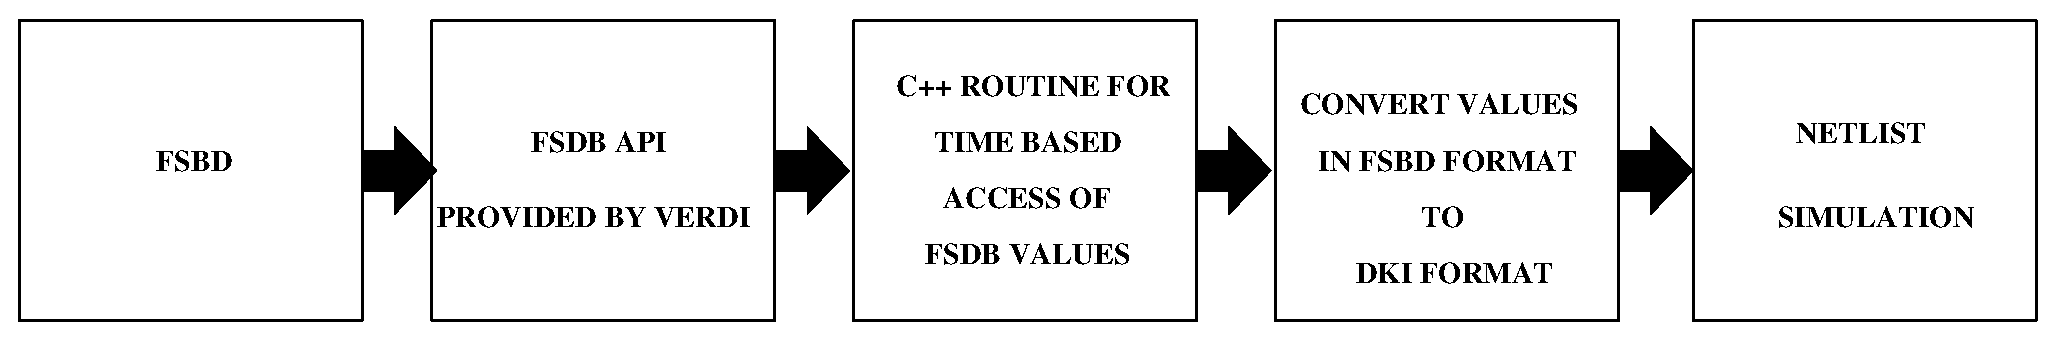
\includegraphics[scale=0.65]{./figures/fsdb.ps}
\caption{Accessing FSDB Signals}
\label{fig:fsdb.ps}
\end{figure}

~\figurename{~\ref{fig:fsdb.ps}} shows how test vectors are obtained from .fsdb file and attached onto the netlist simulation flow. The various stages involved are explained below.

\paragraph{Extracting data from FSDB:}In FSDB signals are stored in binary format and can be accessed only by specific tools or using some appropriate APIs.  In this project we are using FSDB APIs provided by Verdi. These API's allow us to access each signal separately. 


\begin{figure}[h]
\centering
\includegraphics[width=4.5in, height=3.5in]{./figures/verdi.ps}
\caption{API For Accessing FSDB Signals}
\label{fig:verdi.eps}
\end{figure}






Once the list of RTL signals that need to be extracted is decided, make FSDB signals object handles corresponding to each signal. FSDB signal objects are also defined by the API and allow signals in FSDB file to be attached to these objects. Special "{\emph Attach()}" routines are provided for signal attach with objects.

However just attaching to the signal is not enough. A larger C++ infrastructure is required for accessing signals for gatesim because of the following reasons:
\begin{enumerate}
\item Values contained in FSDB needs to be accessed in time-based fashion.
\item Typical netlist contained hundreds of stimulus points with many wider bus-signals.
\end{enumerate}
The C++ infrastructure will open the FSDB file and initiate a playback through the file. Whenever a signal that is attached using APIs changes, the C++ will identify this and will ensure the changed value is made available to the netlist simulation.  Figure x shows the complete flow of the C++ routine developed for FSDB signal access, conversion and application onto Verilog component.


\begin{figure}[h]
\centering
\includegraphics[width=6in]{./figures/cpp.ps}
\caption{C++ Routine for FSDB Signal Extraction}
\label{fig:cpp.eps}
\end{figure}




A set of RTL signal accessed at time based manner and applied onto netlist is effectively doing the job of test vectors as vectors are nothing but signal values at different instants of time.
Once signals are accessed from FSDB file by API's and C++ routine developed next step is applying it onto netlist. However Verilog based netlist cannot directly interact with extracted FSDB format objects. For this a conversion stage is required.  




\paragraph{Convert FSDB format to DKI format}: The FSDB format signals are converted to a standard format that can work with Verilog. There are many interfaces that allow Verilog-C interaction such as PLI, VPI (or PLI 2.0) or DKI. 
In this work we are using DKI which is an API that is supported only by VCS. This has the advantage of less simulation overhead and smaller memory footprint compared to VPI interface.
For converting FSDB signal format to DKI format, we are assigning signal values of the FSDB signal object to a corresponding DKI signal object. Similar to the creation of FSDB signal object list, create a DKI object list corresponding to the RTL signals. 

\begin{figure}[h]
\centering
\includegraphics[width=3.5in, height=3in]{./figures/dki.ps}
\caption{FSDB Format to DKI format}
\label{fig:dki.eps}
\end{figure}



Whenever the C++ moves in time and identify a change in signal value in FSDB signal, an assign statement will assign the new FSDB signal value to DKI signal object.  These DKI signals can drive Verilog signals by using "{\emph Attach}" routine provided by API, that ties together DKI object with RTL signal. 

In the previous section we have discussed extracting FSDB, accessing it in a time based manner and converting it to a format that can interact with Verilog. Next step is using these signals for netlist simulation.

%Features of Improved gatesim methodology are:
%\begin{enumerate}
%	\item Obtain test vectors from FSDB; access it in time-based fashion.
%	\item Drive stimulus onto a dummy RTL. This dummy RTL does not have any logic other than Input/output. All the input and output ports of the module netlist are included in this dummy RTL module. 
%	\item Dummy RTL drives netlist stimulus and other stimulus points inside design (like fuses, un init flops).
%	\item Apply appropriate force signals from FSDB directly on to the dummy RTL. The dummy RTL signal forces the netlist signals.
%	\item Accomplish verification goals by cycle-comparing netlist behavior to that of its counterpart RTL (as available in the FSDB).
%\end{enumerate}
%It should be noted that the improved methodology is still dependent on vectors from RTL simulations and is not independent by itself. But gains obtained in turn-around times were of great benefit.
%


